\section{Требования к программе}

Программа состоит из двух основных компонент: клиентской и серверной частей, между которыми должно быть налажено
взаимодействие.

\subsubsection{Требования к клиентской части}
Клиент должен иметь интерфейс, позволяющий пользователю взаимодействовать с программой с минимальной предварительной
подготовкой.
Дизайн интерфейса должен соответствовать современным тенденциям, обладать адаптивностью под различные характеристики
экранов.
Интерфейс должен менять свой стиль в зависимости от времени суток для имитации освещения в комнате.

Клиент реализует три основных экрана.
На каждом экране расположен свой набор элементов:\\

На главной странице:
\begin{enumerate}[noitemsep]
    \item Поле для ввода ссылки на сторонний видео-ресурс (YouTube, VK, Rutube).
    Поле должно быть «универсальным» для всех ресурсов.
    \item Поле для загрузки файла (.torrent или обычного видео-формата).
    \item Статистика: количество активных пользователей, количество запущенных комнат.
    \item Ссылки на социальные сети проекта;
    \item Кнопка доната, топ донатов за неделю, топ донатов за месяц.
\end{enumerate}

На странице комнаты:
\begin{enumerate}[noitemsep]
    \item Аккаунт пользователя.
    \item Ссылка для подключения к комнате.
    \item Список участников комнаты.
    \item Информация об обработке видео:
    \begin{enumerate}
        \item Процент загрузки;
        \item Процент обработки;
        \item Длительность;
        \item Максимальное качество.
    \end{enumerate}
    \item Дополнительные параметры для видео:
    \begin{enumerate}
        \item Возможность добавить аудиодорожку к видеофайлу;
        \item Возможность добавить субтитры к видеофайлу.
    \end{enumerate}
    \item Дополнительные параметры для комнаты:
    \begin{enumerate}
        \item Возможность добавить ещё одно видео в очередь просмотра;
        \item Настройка прав на добавление аудиодорожен:
        \begin{enumerate}
            \item только создатель;
            \item все пользователи;
            \item выбранные пользователи;
        \end{enumerate}
        \item Настройка прав на перемотку/остановку/возобновление видео:
        \begin{enumerate}
            \item только создатель;
            \item все пользователи;
            \item выбранные пользователи.
        \end{enumerate}
    \end{enumerate}
    \item Текстовый чат пользователей с возможностью его чтения и отправки сообщений.
    \item Проигрыватель с видео.
\end{enumerate}

В проигрывателе с видео:
\begin{enumerate}[noitemsep]
    \item Кнопка изменения качества видео.
    \item Возможность изменения аудиодорожки в процессе просмотра, если есть такая возможность.
    \item Возможность включения/отключения/изменения субтитров, если есть такая возможность.
    \item Возможность тремя способами отправлять сообщения в чат прямо из плеера, не выходя из полноэкранного режима:
    \begin{enumerate}
        \item Обычный текстовый ввод сообщений;
        \item Ввод сообщений посредством голоса с последующим переводом голоса в текстовый вид;
        \item Отправка «реакций» в виде стикеров для быстрых эмоций.
    \end{enumerate}
    \item Отображение сообщений чата прямо в плеере.
    Чат может содержать текстовые сообщения и «реакции».
\end{enumerate}

\newpage

\subsubsection{Требования к серверной части}
На серверной части должен быть реализован алгоритм по преобразованию единого видеоролика в набор видеороликов меньшей длительности
(сегментов).
Также требуется добавить конвертацию видеоролика в видеоролики с меньшим качеством (Рис.~\ref{ris:server_converting}).

Должно быть реализовано взаимодействие с базой данных для хранения данных о комнатах.

\begin{figure}[h]
    \centering
    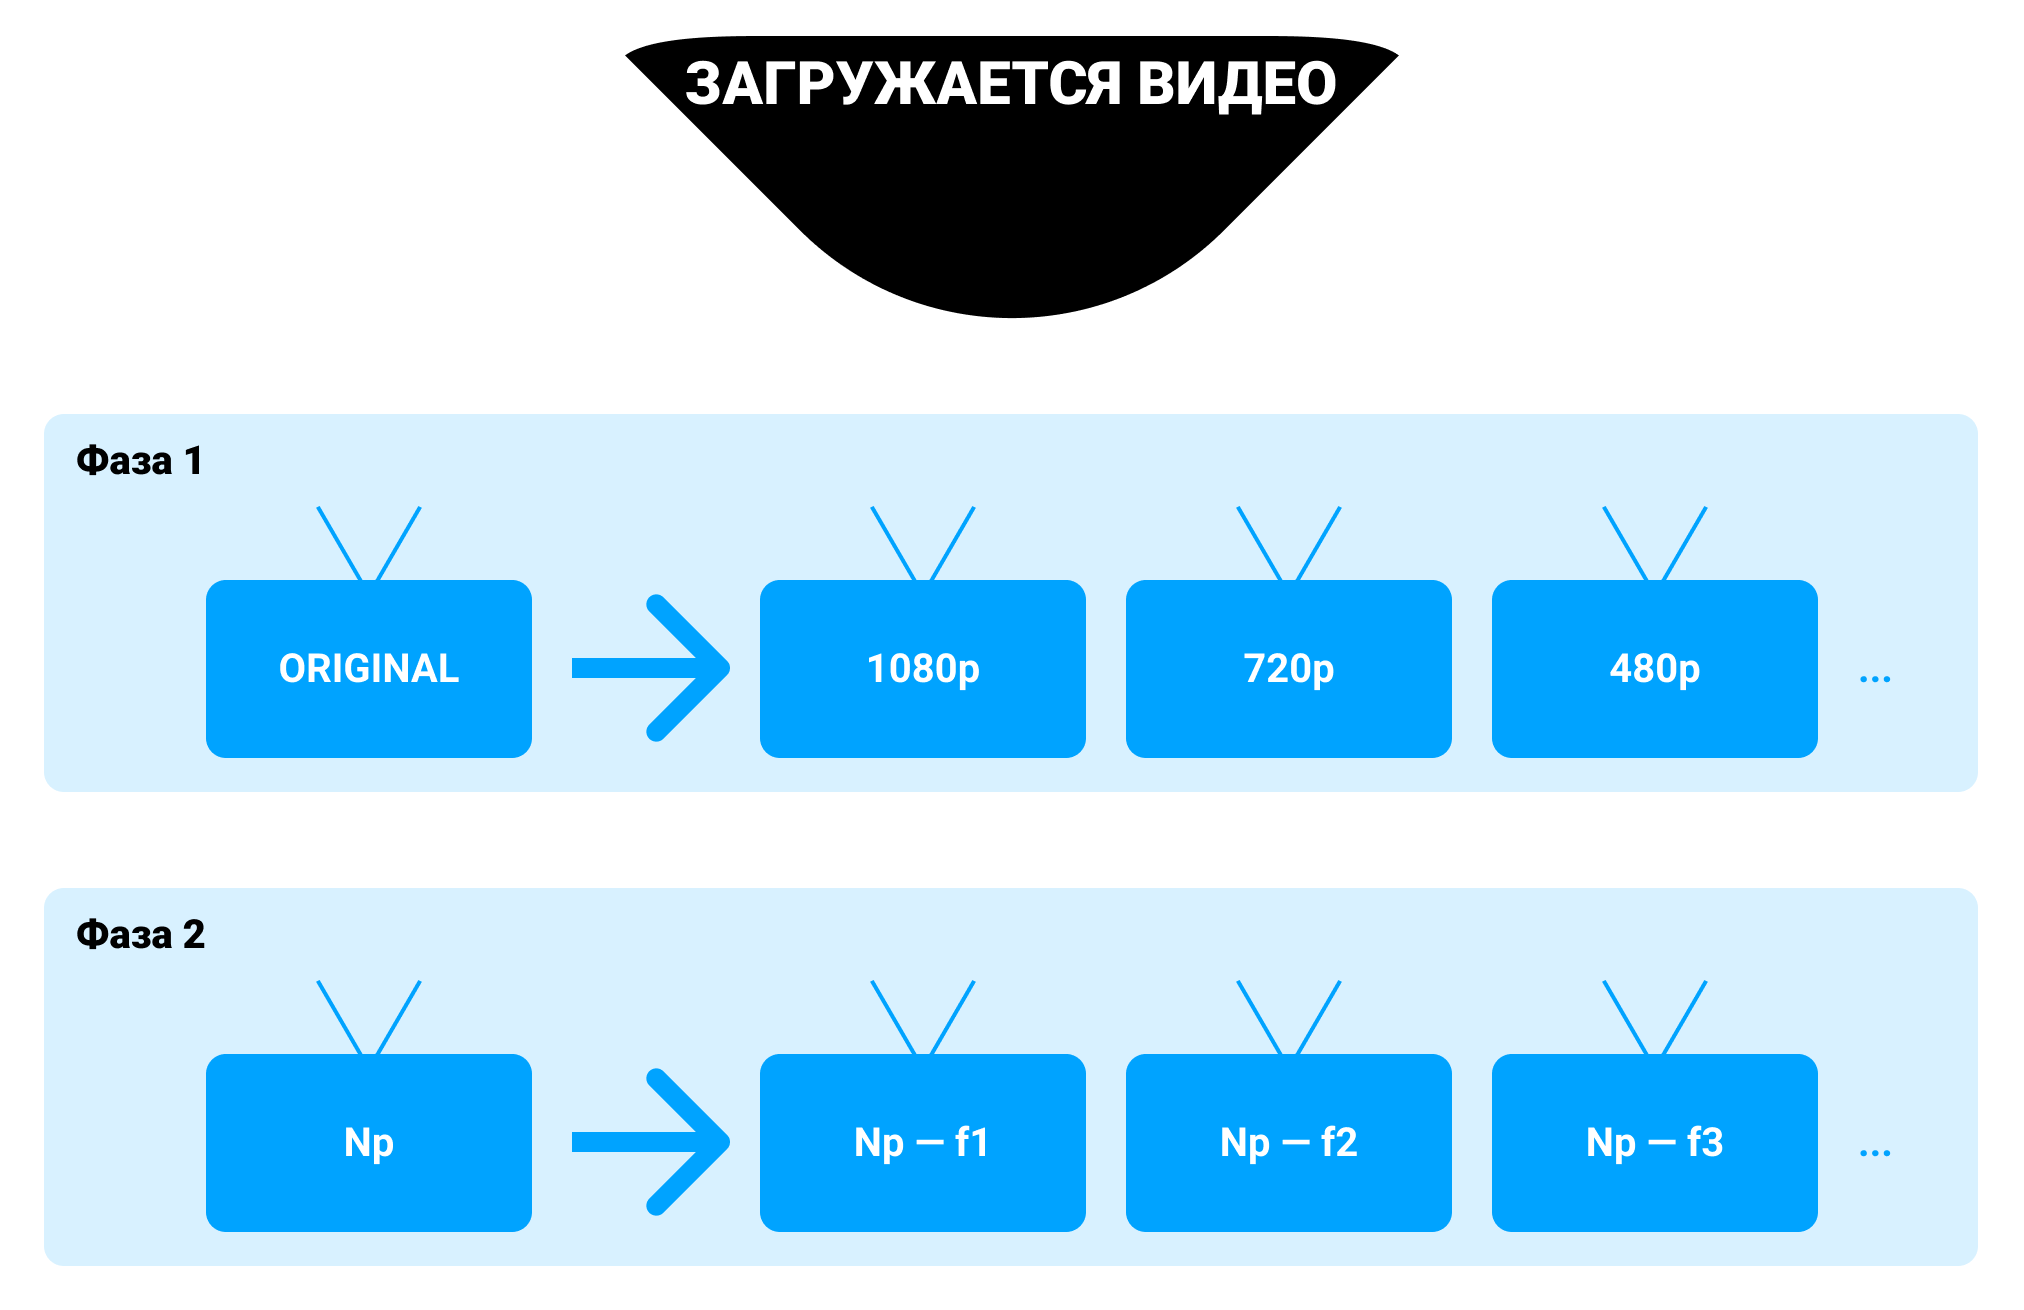
\includegraphics[width=1\linewidth]{images/server_converting.png}
    \caption{Алгоритм конвертации видео}
    \label{ris:server_converting}
\end{figure}

\newpage

\subsubsection{Требования к взаимодействию клиентской и серверной частей}
Взаимодействие между клиентом и сервером должно осуществляться посредством HTTP-запросов и WebSocket-подключений.

При получении HTTP-запроса (GET, POST, UPDATE, DELETE и т.д.) от клиента, сервер должен ответить сообщением в формате
JSON, содержащим необходимую информацию для работы клиента.

Для синхронизации видеопотока между разными клиентами используется протокол WebSocket.
В целях обеспечения наименьшей рассинхронизации видеопотока между клиентами, требуется хранить переменные \(diff\_sc\) и \(diff\_cs\) для
каждого клиента.
Данные переменные будут содержать в себе информацию о количестве затрачиваемого времени при передаче данных от сервера к клиенту или от клиента к серверу.

Формула для определения переменных \(diff\_sc\) и \(diff\_cs\): \begin{gather*}
                                                                    diff\_sc = time\_sc_2 - time\_sc_1\\
                                                                    diff\_cs = time\_cs_2 - time\_cs_1
\end{gather*}, где:
\begin{itemize}[noitemsep]
    \item[--] \(time\_sc_1\) — время отправки сообщения сервером;
    \item[--] \(time\_sc_2\) — время получения сообщения клиентом;
    \item[--] \(diff\_sc\) — разница между временем отправки и временем получения при передаче сообщения от сервера к клиенту;
    \item[--] \(time\_cs_1\) — время отправки сообщения клиентом;
    \item[--] \(time\_cs_2\) — время получения сообщения сервером;
    \item[--] \(diff\_cs\) — разница между временем отправки и временем получения при передаче сообщения от клиента к серверу.
\end{itemize}

Так как возможно подключение нескольких клиентов, требуется хранить содержимое значений \(diff\_sc_i\) и \(diff\_cs_i\) для всех \(n\) клиентов.

Алгоритм (Рис.~\ref{ris:interaction_format}) синхронизации видео единый:
\begin{enumerate}
    \item Клиент \(k\) отправляет серверу запрос на действие \(d\) (перемотку/приостановку/возобновление) видео.
    \item Сервер отправляет всем клиентам сообщение с текущим серверным временем.
    Клиенты принимают значение и считают разницу \(diff\_sc_i\) с учётом своего времени.
    Затем клиенты отправляют посчитанную разницу времени в миллисекундах обратно серверу, а также отправляют текущее клиентское время.
    С учётом полученной информации сервер считает разницу \(diff\_cs_i\).
    \item Сервер отправляет всем клиентам команду выполнить действие \(d\) и передаёт каждому клиенту задержку \(delay_i\),
    которая считается по формуле: \[ delay_i = \max(diff\_sc_1, \ldots, diff\_sc_n) - diff\_sc_i + diff\_cs_k, \;\;\; i \in [1, \ldots, n] \]
\end{enumerate}

Значение \(delay_i\) требуется по-разному использовать в различных ситуациях.
При организации совместного просмотра фильма возможны следующие сценарии:
\begin{itemize}
    \item[--] \textbf{Перемотка} видео на позицию \(t\) мс одним из клиентов.

    При получении такой команды все клиенты (кроме клиента-инициатора) выполняют перемотку видео на позицию \((t + delay_i)\) мс.
    \item[--] \textbf{Приостановка} видео одним из клиентов.

    При получении такой команды все клиенты (кроме клиента-инициатора) выполняют перемотку видео на \(delay_i\) мс назад.
    \item[--] \textbf{Возобновление} видео одним из клиентов.

    При получении такой команды все клиенты (кроме клиента-инициатора) выполняют перемотку видео на \(delay_i\) мс вперёд.
\end{itemize}

\begin{figure}[h]
    \centering
    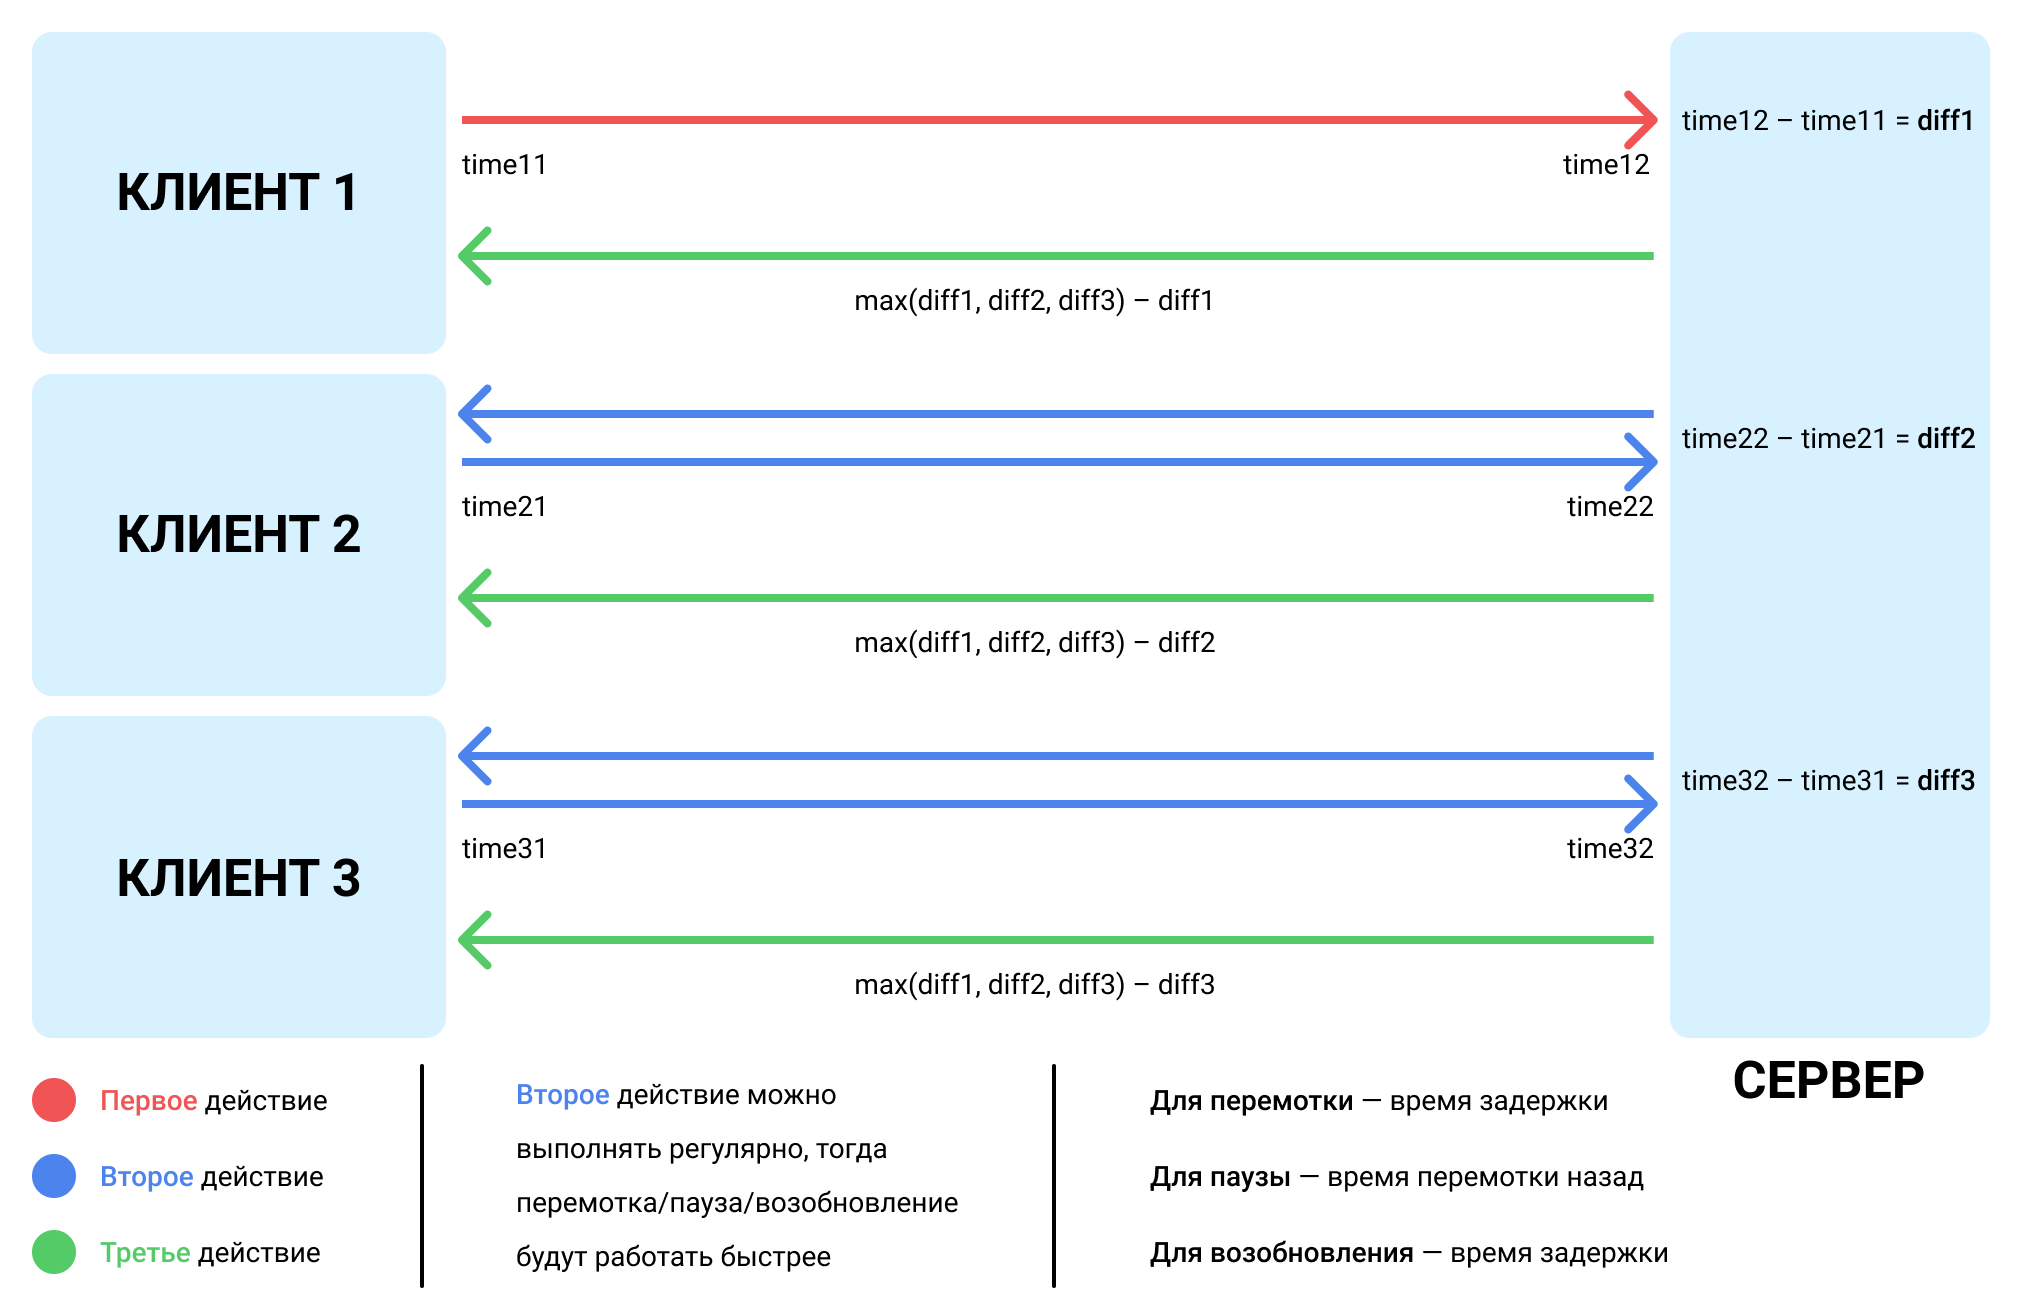
\includegraphics[width=1\linewidth]{images/interaction_format.png}
    \caption{Алгоритм синхронизации видеопотока}
    \label{ris:interaction_format}
\end{figure}

\newpage

\subsubsection{Требования к организации входных данных}
Входные данные программы должны быть организованы в виде вводимого в специальную форму текста или файла,
соответствеющего определённому шаблону.
Данные, вводимые вручную, проверяются на корректность после попытки сохранения;
данные, вводимые из файла, проверяются в ходе анализа и размещения данных.

\subsubsection{Требования к организации выходных данных}
Выходные данные программы должны быть организованы в виде визуальных эффектов интерфейса, текстов, картинок и
видеороликов, расположенных на WEB-странице.

Видеоролики должны делиться на фрагменты, которые в последствии WEB-проигрыватель должен склеивать в полноценное видео.

\subsection{Требования к надёжности}

\subsubsection{Требования к обеспечению надёжного (устойчивого) функционирования программы}

Разрабатываемый сервер должен:
\begin{enumerate}
    \item запрещать доступ к REST API методам для неавторизованных пользователей;
    \item быть устойчивым к атакам следующего типа:
    \begin{enumerate}
        \item Cross-Site Scripting (XSS),
        \item SQL Injection,
        \item Local File Inclusion (LFI),
        \item Distributed Denial of Service (DDoS).
    \end{enumerate}
\end{enumerate}

\subsubsection{Время восстановления после отказа}
Время восстановления после отказа, вызванного сбоем электропитания технических средств (иными внешними факторами),
не фатальным сбоем (не крахом) операционной системы, не должно превышать времени, необходимого на перезагрузку
операционной системы и запуск программы, при условии соблюдения условий эксплуатации технических и программных средств.

Время восстановления после отказа, вызванного неисправностью технических средств, фатальным сбоем (крахом) операционной
системы, не должно превышать времени, требуемого на переустановку программных средств.

\subsubsection{Отказы из-за некорректных действий оператора}
Во избежание возникновения отказов программы по причине некорректных действий оператора следует обеспечить работу
конечного пользователя без предоставления ему административных привилегий.

\subsection{Условия эксплуатации}

Для корректной эксплуатации системы необходим системный администратор, знакомый с языком программирования
Java, а также СУБД PostgreSQL.

Прочие требования эксплуатации приложения определяются требованиями к условиям эксплуатации технических средств.

\subsection{Требования к составу и параметрам технических средств}

В состав технических средств сервера должен входить компьютер или система компьютеров.
Допускается использование облачных сервисов.

Рекомендуется следующие характеристики:
\begin{enumerate}
    \item Объём оперативной памяти 8 Гб;
    \item Объём физической памяти не менее 50 Гб.
\end{enumerate}

\subsection{Требования к информационной и программной совместимости}

\subsubsection{Требования к исходным кодам и языкам программирования}

Исходные коды для сервера должны быть реализованы с использованием следующих языков и технологий:
\begin{enumerate}[noitemsep]
    \item Java;
    \item Spring Boot — для реализации базовой архитектуры сервера;
    \item Spring Web — для реализации REST API методов и панели администрирования;
    \item Spring Thymeleaf — для миграций и версионирования базы данных;
    \item Hibernate — для работы с базой данных, для связки таблиц базы данных с классами Java;
    \item ffmpeg — для обработки видеофайлов: нарезка и изменение качества;
    \item PostgreSQL — использовать в качестве СУБД;
    \item Docker, docker-compose — для обеспечения переносимости сервера.
\end{enumerate}

\subsubsection{Требования к программным средствам, используемым программой}
Требования к информационным и программным характеристикам сервера:
\begin{enumerate}[noitemsep]
    \item Наличие доступа по SSH;
    \item Открытые порты: 22, 40, 80, 443, 3000, 5432, 5454, 8080-8100;
    \item Установленные утилиты: nano, apt-get;
    \item Установленные: docker, docker-compose, docker-machine;
    \item Установленный с настройками по-умолчаию: Nginx, пользователь с доступом по SSH должен иметь права
    на редактирование конфигурации;
    \item Операционная система Ubuntu 16.04.
\end{enumerate}

\subsection{Требования к маркировке и упаковке}

Сервер должен быть удалённо развёрнут на одном из облачных сервисов.
Для обеспечения переносимости требуется настроить контейнер Docker.